\subsection{Diagrama de clases del sistema}

Con el objetivo de definir la estructura estática del sistema, se presenta el diagrama de clases, el cual describe las principales entidades, sus atributos y las relaciones existentes entre ellas.

\begin{figure}[H]
    \centering
    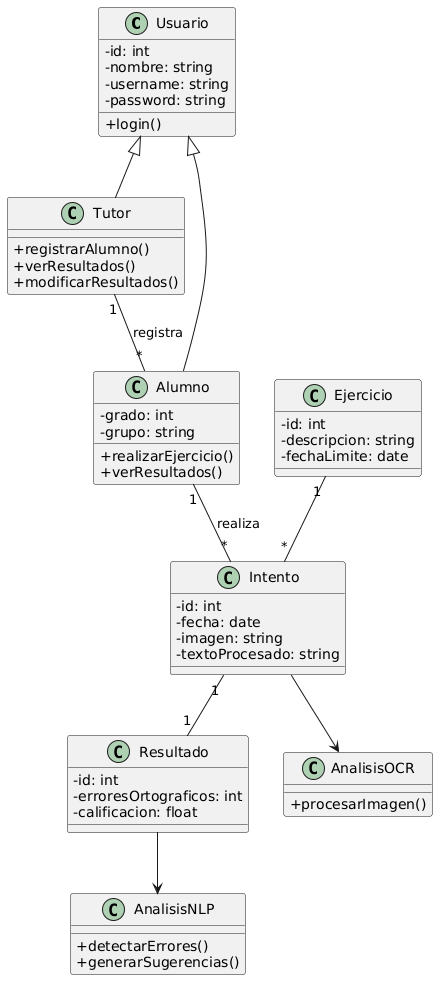
\includegraphics[width=0.60\textwidth]{Imagenes/DiagramaDeClases.png}
    \caption{Diagrama de clases del sistema}
    \label{fig:diagrama_clases}
\end{figure}

El diagrama de clases representa la estructura estática del sistema, mostrando las principales entidades, sus atributos y las relaciones entre ellas. Se observa una jerarquía de herencia donde la clase \textit{Usuario} es la base para los actores \textit{Tutor} y \textit{Alumno}. Asimismo, se modelan los elementos centrales del sistema como \textit{Ejercicio}, \textit{Intento} y \textit{Resultado}, los cuales permiten gestionar el proceso de captura, análisis y retroalimentación de la escritura. Finalmente, se integran los módulos de procesamiento \textit{AnalisisOCR} y \textit{AnalisisNLP}, responsables de la conversión de imágenes a texto y la detección de errores ortográficos respectivamente.

%------------------------------------------------

\subsection{Diagrama de secuencia del procesamiento de ejercicios}

Con el propósito de representar el comportamiento dinámico del sistema, se presenta el diagrama de secuencia correspondiente al proceso de análisis de ejercicios, el cual describe la interacción entre los diferentes componentes involucrados desde la captura de la imagen hasta la generación de resultados.

\begin{figure}[H]
    \centering
    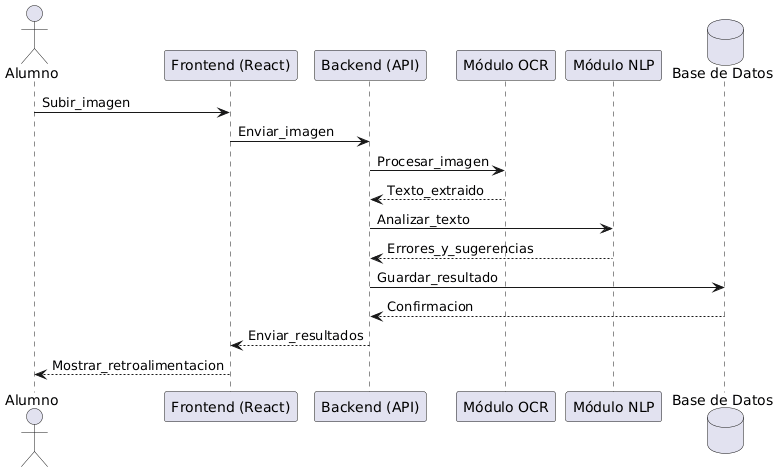
\includegraphics[width=0.75\textwidth]{Imagenes/DiagramaDeSecuencia.png}
    \caption{Diagrama de secuencia del procesamiento de ejercicios}
    \label{fig:diagrama_secuencia}
\end{figure}

El diagrama muestra cómo el alumno interactúa con la interfaz para enviar una imagen, la cual es procesada por el backend mediante un módulo OCR para la extracción de texto. Posteriormente, el texto es analizado por el módulo NLP para identificar errores ortográficos y generar sugerencias. Finalmente, los resultados son almacenados en la base de datos y enviados al usuario para su visualización.

%------------------------------------------------

\subsection{Diagrama de actividad del procesamiento de ejercicios}

Con el propósito de representar el flujo de actividades del sistema, se presenta el diagrama de actividad correspondiente al proceso de análisis de ejercicios, el cual describe de manera secuencial las acciones realizadas desde la interacción del usuario hasta la generación de resultados.

\begin{figure}[H]
    \centering
    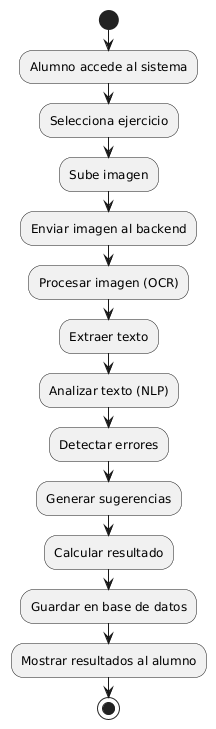
\includegraphics[width=0.35\textwidth]{Imagenes/DiagramaDeActividad.png}
    \caption{Diagrama de actividad del procesamiento de ejercicios}
    \label{fig:diagrama_actividad}
\end{figure}

El diagrama muestra la secuencia de actividades que se llevan a cabo cuando un alumno realiza un ejercicio, comenzando desde la selección y envío de la imagen, pasando por el procesamiento mediante OCR y el análisis con técnicas de procesamiento de lenguaje natural, hasta la generación y almacenamiento de los resultados, los cuales son finalmente presentados al usuario.

%------------------------------------------------

%\subsection{Diagrama de estados del proceso de evaluación}

%Con el propósito de representar los diferentes estados por los que pasa un ejercicio dentro del sistema, se presenta el diagrama de estados, el cual describe el ciclo de vida del proceso de evaluación desde su inicio hasta la presentación de resultados.

%\begin{figure}[H]
%    \centering
%    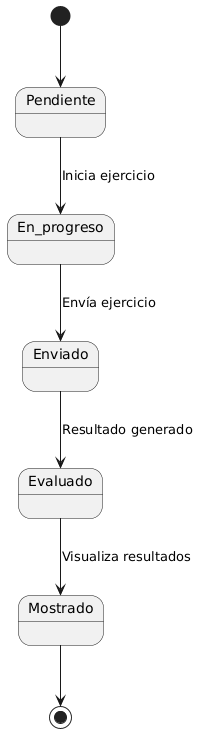
\includegraphics[width=0.60\textwidth]{Imagenes/DiagramaDeEstado.png}
%    \caption{Diagrama de estados del proceso de evaluación}
%    \label{fig:diagrama_estados}
%\end{figure}

%El diagrama muestra los estados principales por los que transita un ejercicio dentro del sistema, desde que se encuentra pendiente, pasando por su desarrollo y envío, hasta su evaluación y visualización por parte del usuario. Este modelo permite comprender el comportamiento general del sistema durante el proceso de evaluación sin detallar los procesos internos.
            
%------------------------------------------------

\subsection{Diagrama de componentes del sistema}

Con el objetivo de representar la estructura modular del sistema, se presenta el diagrama de componentes, el cual muestra la organización de los principales elementos de software y sus interacciones dentro de la arquitectura de la aplicación.

\begin{figure}[H]
    \centering
    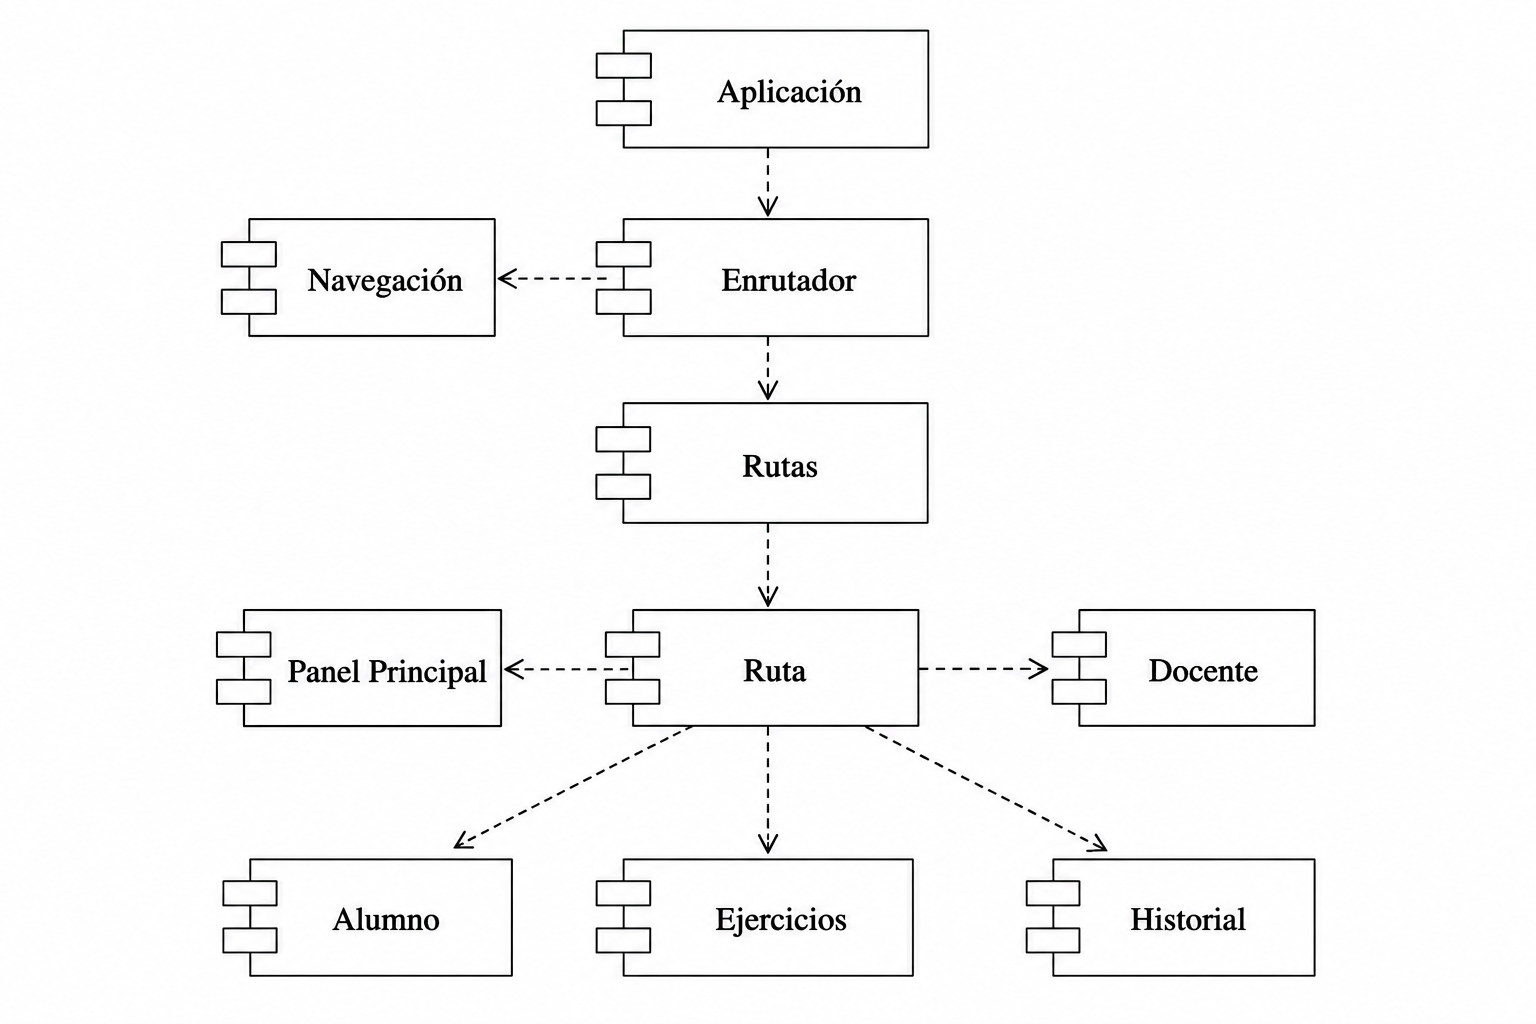
\includegraphics[width=0.65\textwidth]{Imagenes/DiagramaDeComponentess.png}
    \caption{Diagrama de componentes del sistema}
    \label{fig:diagrama_componentes}
\end{figure}

El diagrama muestra la separación del sistema en tres capas principales: cliente, servidor y persistencia. El frontend se encarga de la interacción con el usuario, mientras que el backend gestiona la lógica del sistema y coordina el procesamiento mediante los módulos OCR y NLP. Finalmente, la base de datos permite almacenar la información generada y consultada durante la operación del sistema.

La separación de los módulos de procesamiento OCR y NLP permite una arquitectura más flexible y escalable, ya que cada componente puede ser optimizado o actualizado de manera independiente. Además, esta división facilita el mantenimiento del sistema y mejora la eficiencia en el procesamiento de la información.

%------------------------------------------------

\subsection{Diagrama de despliegue del sistema}

Con el objetivo de representar la distribución física del sistema, se presenta el diagrama de despliegue, el cual muestra los nodos de hardware involucrados y la forma en que los componentes de software se encuentran distribuidos dentro de la arquitectura de la aplicación.

\begin{figure}[H]
    \centering
    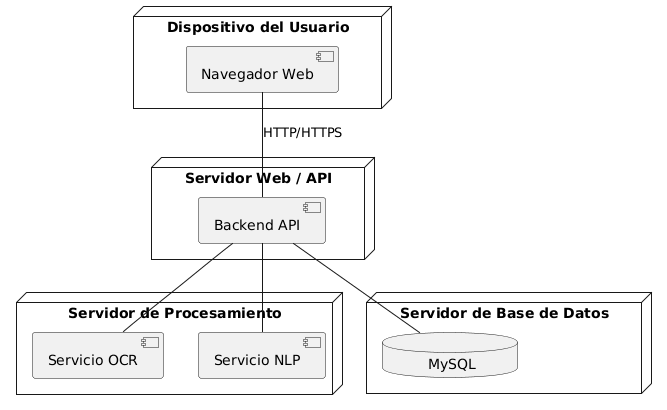
\includegraphics[width=0.65\textwidth]{Imagenes/DiagramaDeDespliegue.png}
    \caption{Diagrama de despliegue del sistema}
    \label{fig:diagrama_despliegue}
\end{figure}

El diagrama muestra la organización del sistema en distintos nodos físicos, incluyendo el dispositivo del usuario, el servidor de aplicaciones, el servidor de procesamiento y el servidor de base de datos. En el dispositivo del usuario se ejecuta el navegador web, desde donde se realizan las solicitudes al backend mediante protocolos HTTP/HTTPS. El servidor de aplicaciones gestiona la lógica del sistema, mientras que los servicios de procesamiento OCR y NLP se encargan de analizar la información recibida. Finalmente, el servidor de base de datos permite almacenar y consultar la información generada durante la operación del sistema.

Asimismo, se observa la separación de los servicios en distintos nodos, lo cual permite una mejor distribución de la carga y facilita la escalabilidad del sistema.